\documentclass[12pt,two column]{article}

\usepackage{graphicx}
\graphicspath{{Documents/}}
\begin{document}
\title{ASSIGNMENT NO.1  \\COURSE CODE-AI1110\\ Probability And Random Variables }
\author{NAME-Abhishek Kumar ROLL NO.=AI21BTECH11003}
\maketitle

\section*{ Question 1a}
 Solve the following inequation and write down the solution set:\\
11x-4$<$15x+4$\le$13x+14,x belongs to W\\
Represent the solution on number line .

 \section*{Solution}

There are two inequatilities.\\

Lets solve for left inequation.

11x-4$<$15x+4\\
$\Rightarrow$ -8$<$15x-11x\\
$\Rightarrow$-2$<$x\\

 Lets solve for right inequation.\\
 15x+4$\le$13x+14\\
$\Rightarrow$ 2x$\le$10\\
$\Rightarrow$x$\le$5\\

-2$<$x$\le$5\\


x belongs to W\\
$\Rightarrow$ $x=0,1,2,3,4,5$ is the required solution

\begin{figure}

This plot shows three lines :\\
y=11x-4,
y=15x+4,
y=13x+14.
\\Red stars are solution points trapped between x=-2 and x=5 on number line y=0 verifying our solution.
\includegraphics[scale=0.5]{figure_2.png}
\end{figure}

\begin{figure}
THIS PLOT REPRESENTS A NUMBER LINE WITH REQUIRED SOLIUTION POINTS.

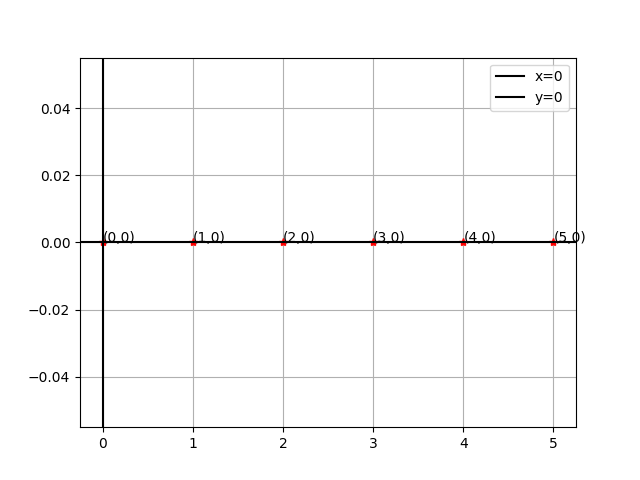
\includegraphics[scale=1]{Figure_1}
\end{figure}


\end{document}
